% !TeX encoding = UTF-8
% !TeX spellcheck = en_US
% !TeX root = presentation.tex
\subsection{KUKA youBot}
\begin{frame}{youBot Driver}
    \begin{itemize}
        \item Drive base
        \item Laser scanners
        \item Arm 
        \item Joystick
        \item Camera
        \item Transformations
        
    \end{itemize}
\end{frame}
\begin{frame}{Map building II}
\end{frame}
\begin{frame}{Map building III}
    \centering
    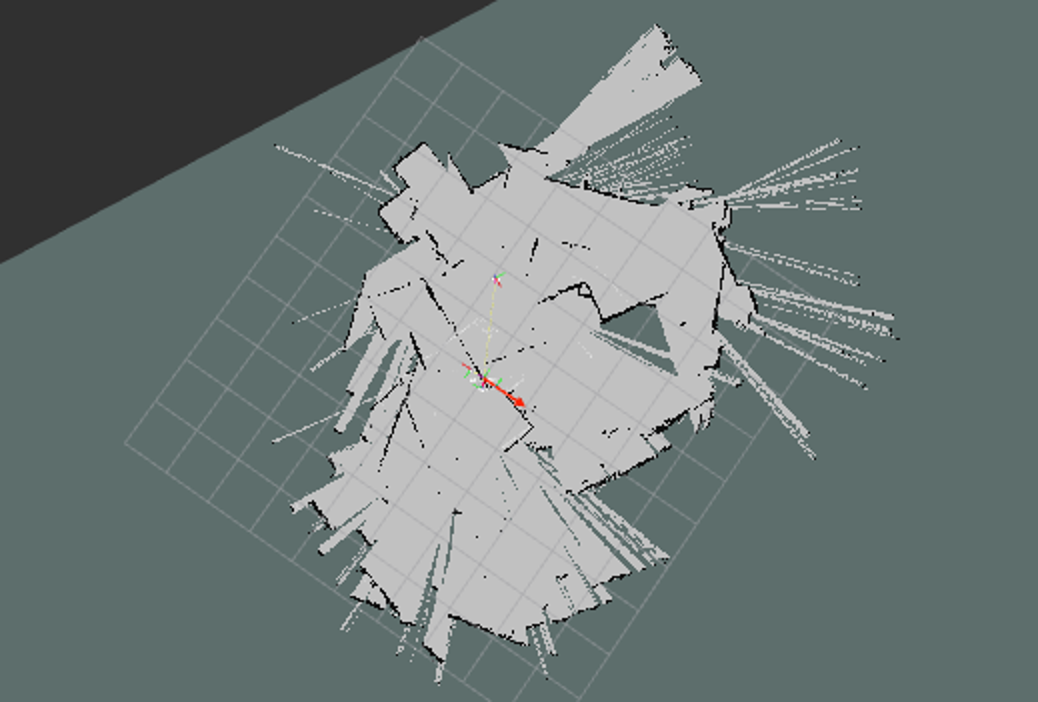
\includegraphics[width=0.9\textwidth]{gfx/map_messy.png}
\end{frame}
\begin{frame}{Localization II}
\end{frame}
\begin{frame}{Navigation}
\end{frame}
\begin{frame}{Navigation - Local Planner}
\end{frame}
\begin{frame}{BNT.py}
    
    The node acts as path executor that reads  a set of user inputs and convert them to move\_base\_msgs.
    \begin{itemize}
        \item Class: Position, Pose, Environment, Workspace, PathExecutor
        
        \item Functions:
        \begin{itemize}
            \item 
            \item Clear cost map
            \item 
        \end{itemize}
    \end{itemize}
    
\end{frame}
